%% PNAStwoS.tex
%% Sample file to use for PNAS articles prepared in LaTeX
%% For two column PNAS articles
%% Version1: Apr 15, 2008
%% Version2: Oct 04, 2013

%% BASIC CLASS FILE
\documentclass{pnastwo}

%% ADDITIONAL OPTIONAL STYLE FILES Font specification

%\usepackage{pnastwoF}



%% OPTIONAL MACRO DEFINITIONS
\def\s{\sigma}
%%%%%%%%%%%%
%% For PNAS Only:
\url{www.pnas.org/cgi/doi/10.1073/pnas.0709640104}
\copyrightyear{2008}
\issuedate{Issue Date}
\volume{Volume}
\issuenumber{Issue Number}
%\setcounter{page}{2687} %Set page number here if desired
%%%%%%%%%%%%

\begin{document}

\title{Coevolution leaves a stronger imprint on interactions than on community structure}

\author{Timoth\'ee Poisot\affil{1}{School of Biological Sciences, University of Canterbury, Christchurch, New Zealand}
\affil{2}{Département des Sciences Biologiques, Université de Montréal, Montréal, Canada}
\affil{3}{Québec Centre for Biodiversity Sciences, Montréal, Canada}\and
Daniel B. Stouffer\affil{1}{}}

\contributor{Submitted to Proceedings of the National Academy of Sciences
of the United States of America}

%%%Newly updated.
%%% If significance statement need, then can use the below command otherwise just delete it.
\significancetext{Every ecological community is ultimately the outcome of evolutionary and coevolutionary processes in the past and ecological processes in the present. Previous studies have described the way that extant interactions can be captured by knowing species' evolutionary relationships while failing to quantify whether coevolution between these species underpins this observation. Here, we demonstrate how the fingerprint of coevolution is eroded away by distinct ecological processes, but also show that this signal is most manifest in interactions as opposed to whole networks. This implies that network structure is the most parsimonious mechanism by which coevolution proceeds and not the imprint it leaves on ecological communities.}

\maketitle

\begin{article}
\begin{abstract}
{Coevolutionary dynamics act on both species and their interactions in
ways that shape ecological communities. It remains unclear, however, how
the structure of communities at larger spatial scales either influences
or is influenced by local coevolutionary processes, and how mechanisms
acting at these different scales feedback onto one another. Here we show
that, although species interactions vary substantially over a
continental gradient, the coevolutionary significance of individual
interactions is maintained across different scales. Notably, this occurs
despite the fact that observed community variation at the local scale
frequently tends to weaken or remove community-wide coevolutionary
signal. When considered in terms of the interplay between community
ecology and coevolutionary theory, our results demonstrate that
individual interactions are capable and likely to show a consistent
signature of past coevolution even when woven into communities that do
not.}
\end{abstract}

\keywords{coevolution | host--parasite interactions | ecological networks | community ecology}

\abbreviations{PACO, Procrustean Approach to Cophylogeny}

\dropcap{E}cological interactions often exert important selective pressures on the
species involved. For example, the phenologies of lodgepole pines and
red crossbills respond spatially to the presence of squirrels
\cite{benk03a} and palm species undergo changes in seed morphology in
response to the extinction of bird dispersing their seeds
\cite{gale13}. Given that interactions are distributed in similar ways
across communities, at both the large or small scale \cite{jord03}, it
can be argued that much ecological structure is the end result of
evolutionary or coevolutionary dynamics between species
\cite{eklo11, stou12}. Unfortunately, while the coevolutionary dynamic
of pairs of interacting species has been well described at macro
\cite{van73} and micro \cite{gand08} evolutionary timescales, most
attempts to understand how they cascade up to the levels of diversity of
both species and interactions found within empirical communities have
been inconclusive \cite{hemb14}. Moreover, because coevolutionary
dynamics are often presented as a key driving force behind ecological
structure across both time and space \cite{thom05}, it is crucial to
determine the scale at which they are both relevant and quantifiable.

Historically, the evidence for coevolution in taxonomically diverse
communities is quantified as the degree of matching between the
phylogenies of two sets of interacting organisms \cite{lege02}. This
notion builds on the century-old idea that extant species interact in a
way similar to the way their ancestors did \cite{fahr13}, but it is
considerably more restrictive than just phylogenetic conservation of
species' interactions \cite{reze07, eklo11} because it additional
higher-order constraints. More explicitly, communities that have
assembled by successive divergence events due to coevolution should
display phylogenetic congruence, that is (i) have similar phylogenetic
trees and (ii) have species at matching positions in the trees that tend
to interact \cite{page03}. On the other hand, many ecological and
evolutionary processes that occur locally are expected to blur
community-wide coevolutionary signal \cite{pois15}. One possible
explanation is that interactions can display substantial turnover at
ecologically relevant temporal and spatial scales \cite{pois12c}: the
same two species can interact in different ways under the effect of
local environmental contingencies, spatial mismatch in species
phenologies, variations in population abundances, and chance events
\cite{pois15a}. It is unclear, however, whether these mechanisms
influence how the coevolutionary signal within individual interactions
should vary across spatial scales.

To answer these questions, we study a dataset of interactions between
rodents and their ectoparasites from 51 sites across Western to Eastern
Europe \cite{kras12b} (Methods). This dataset is uniquely
suited for this task as it represents a paradigmatic system in which
species-species interactions are thought to be driven by macro-evolution
and co-speciation events \cite{vern09}, and coevolutionary signal is
indeed significant at the continental level \cite{kras12a}
(\(p \leq 10^{-4}\); Methods). Importantly, it also provides spatial
replication and variability at a scale large enough to capture
macro-ecological processes.

As host-macroparasite interactions are hypothesized to be both
ecologically constrained and evolutionary conserved \cite{comb01}, the
congruence observed at the continental level sets the baseline for what
would be expected in local communities. Of course, if ecological
mechanisms reduce coevolutionary signal, we should detect coevolution at
the continental scale but not locally. Noting that variation of
interactions can decrease congruence, we analyse the data at two
different levels to test these hypotheses: first, we use \emph{regional}
interaction data---which accounts for different species composition
across sites--and second, we use the \emph{local} interaction
data---which also accounts for variation in the interactions between
observed these species (Methods Summary). Out of 51 sites, 35 show no
signal of coevolution, 11 show significant coevolutionary signal when
using the regional interactions, and 12 show significant coevolutionary
signal using the local interactions (see \emph{Supp. Mat. 1} for
network-level significance values).

These results would appear to support the idea that macro-evolutionary
processes such as co-diversification can have consequences at the
macro-ecological level but may not in fact be detectable at finer
spatial scales. On the other hand, system-level differences say little
about the behaviour of individual interactions, despite the fact most
coevolutionary mechanisms act at the interaction level \cite{thom99}.
As might be expected, we observe here that networks with interactions
that are important for coevolution at the continental scale indeed have
more coevolutionary signal at the local and regional scales alike (Fig.
2A). Intriguingly, we also find that the distribution of individual
interactions' contributions to coevolution is strongly conserved,
regardless of the scale at which the interactions are quantified (Fig.
2B). Because interactions differ in their total contribution to
coevolution, this implies that their distribution across networks is
what actually drives differences in overall coevolutionary signal.
Network-level coevolutionary signal emerges directly from the properties
of interactions and is not a property of the network itself.

Beyond their contribution to coevolution, interactions also ultimately
differ in how frequently they vary when the species involved co-occur
\cite{olit14}. Once more, the literature on host-parasite interactions
usually assumes that the reason why some interactions are more frequent
is because they reflect a significant past history of coevolution
\cite{mora10}. If this were true, we should observe a significant,
positive correlation between the probability of observing an interaction
and the importance of that interaction for coevolution at the
continental scale (Methods Summary). Surprisingly, we find that neither
is true here since interactions that are important for coevolution are
not more conserved (Fig. 3).

Ultimately, coevolutionary signal varies across scale because of the
simultaneous variation of species' interactions \emph{and} communities'
phylogenetic tree structure. In a system characterised by substantial
turnover, we would expect the contribution of each separate interaction
to differ across scales as well. Instead, we observe here that
interactions that contribute strongly to coevolutionary signal at the
continental scale \emph{also} show a significant tendency to contribute
strongly at the local (\(p<0.05\) for positive correlations in 48 out of
51 networks) and regional (in 47 out of 51 networks), and this
observation is independent of network-wide coevolutionary signal (Fig.
4). Remarkably, this result implies that the remnants of coevolution are
still locally detectable in \emph{individual interactions} even though
coevolution regularly fails to leave its imprint on most local networks.

Overall, the results of our analyses demonstrate that there is a
sizeable gap between our current understanding of coevolution as the
basis of multi-species interactions and its applicability to ecological
questions. Local networks show little to no signal of coevolution and
the strength of coevolution between two species is a surprisingly poor
predictor of how frequently they interact. In contrast to the frequent
assumption that phylogenetic structure is a key driver of community
structure \cite{cave09}, these data reveal that this impact is actually
minimal at ecologically relevant spatial scales. Despite all the above,
individual interactions are able to maintain their coevolutionary signal
even when the community they are woven into does not. Thinking more
broadly, these discrepancies provide a clear roadmap for bridging the
aforementioned gap between our appreciation of the role of coevolution
and its empirically measurable outcomes. Network structure is the most
parsimonious \emph{mechanism} by which coevolution proceeds, not the
imprint coevolution leaves on ecological communities.


\begin{materials}
\section{Data provenance} We use data on observations of interactions between 121 species of
rodents and 205 species of parasitic fleas in 51 locations across Europe
\cite{kras12b} to build 51 species-species interaction networks.
Interactions were measured by combing rodents for fleas, a method that
gives high quality data as it has a high power of detection. To account
for differential sampling effort and across site variations in
abundance, we only study the networks' incidence matrices (presence and
absence of interactions).

\section{Spatial scales} In our study, we define threes scales for the network data and
analysis---continental, regional, and local. The continental scale is
the aggregated ``metanetwork'' which includes all potential interactions
between co-occurring species \cite{pois12c} (\emph{i.e.}, all species
and all their interactions across the 51 networks). Within each site,
the regional scale is given by the list of observed species and all
their possible interactions. Hence the regional networks are always a
perfect subset of the continental network. The local scale includes only
the interactions that were actually observed in the field at a given
site. Therefore, the local and regional networks always include the same
species, but the local network has only a subset (or, at most, an exact
match) of the interactions in the regional network. The spatial
consistency of every individual interaction is measured as the number of
sites in which the two species involved co-occur.

\section{Quantifcation of coevolutionary signal} We quantified the coevolutionary signal in terms of the degree of
matching between host and parasite phylogenies given knowledge of
species interactions using the \emph{PACO} method \cite{balb13}, which
is robust to variations in number of species. \emph{PACO} provides
measures of both the network-level congruence (\emph{i.e.}, is the
network coevolved?) and the interaction-level signal (\emph{i.e.}, what
is the contribution of each interaction to the overall coevolutionary
signal?). We measured the phylogenetic dissimilarity between two sites
for hosts and parasites using PCD \cite{ives10}, a measure that
accounts for the dissimilarity of species, corrected for the
phylogenetic distance between all species in the dataset. Since it is a
requirement of the methods we use here, the phylogenetic trees for hosts
and parasites were rendered ultrametric (i.e., all species are at the
same distance from the root).
\end{materials}


\begin{acknowledgments}
We thank Juan Antonio Balbuena for
discussions about the \emph{PACo} method, and members of the Stouffer
and Tylianakis groups for comments on an early draft of this manuscript.
We are indebted to Matt Hutchinson and Fernando Cagua for contributions
to the code of the \texttt{paco} R package. Funding to TP and DBS was
provided by a Marsden Fund Fast-Start grant (UOC-1101) and to DBS by a
Rutherford Discovery Fellowship, both administered by the Royal Society
of New Zealand. TP received additional support through a Starting grant from the 
Universit\'e de Montr\'eal, and through a NSERC Discovery grant.
\end{acknowledgments}

\begin{thebibliography}{10}

\bibitem{benk03a}
Benkman CW, Parchman TL, Favis A, Siepielski AM (2003) Reciprocal selection
  causes a coevolutionary arms race between crossbills and lodgepole pine.
\newblock {\em Am. Nat.} 162(2):182--194.

\bibitem{gale13}
Galetti M et~al. (2013) Functional extinction of birds drives rapid
  evolutionary changes in seed size.
\newblock {\em Science} 340(6136):1086--1090.

\bibitem{jord03}
Jordano P, Bascompte J, Olesen JM (2003) Invariant properties in coevolutionary
  networks of plant-animal interactions.
\newblock {\em Ecol. Lett.} 6(1):69--81.

\bibitem{eklo11}
Eklof A, Helmus MR, Moore M, Allesina S, Ekl{\"o}f A (2011) Relevance of
  evolutionary history for food web structure.
\newblock {\em Proc. R. Soc. B Biol. Sci.} 279(November 2011):1588--1596.

\bibitem{stou12}
Stouffer DB, Sales-Pardo M, Sirer MI, Bascompte J (2012) Evolutionary
  conservation of species' roles in food webs.
\newblock {\em Science} 335(6075):1489--1492.

\bibitem{van73}
Van~Valen L (1973) A new evolutionary law.
\newblock {\em Evol. Theory} 1(1):1--30.

\bibitem{gand08}
Gandon S, Buckling A, Decaestecker E, Day T (2008) Host-parasite coevolution
  and patterns of adaptation across time and space.
\newblock {\em J. Evol. Biol.} 21(6):1861--1866.

\bibitem{hemb14}
Hembry DH, Yoder JB, Goodman KR (2014) Coevolution and the diversification of
  life.
\newblock {\em The American Naturalist} 184(4):425--438.

\bibitem{thom05}
Thompson JN (2005) {\em The Geographic Mosaic of Coevolution}.
\newblock (University Of Chicago Press).

\bibitem{lege02}
Legendre P, Desdevises Y, Bazin E (2002) A statistical test for host-parasite
  coevolution.
\newblock {\em Syst. Biol.} 51(2):217--234.

\bibitem{fahr13}
Fahrenholz H (1913) Ectoparasiten und abstammungslehre.
\newblock {\em Zool. Anz.} 41:371--374.

\bibitem{reze07}
Rezende EL, Lavabre JE, Guimar{\~a}es PR, Jordano P, Bascompte J (2007)
  Non-random coextinctions in phylogenetically structured mutualistic networks.
\newblock {\em Nature} 448(7156):925--8.

\bibitem{page03}
Page RDM (2003) {\em Tangled trees: Phylogeny, cospeciation, and coevolution}.
\newblock (University of Chicago Press).

\bibitem{pois15}
Poisot T (2015) When is cophylogeny evidence of coevolution? in {\em
  Evolutionary Ecology of Host-Parasite Systems}, eds.{} Morand S, Littlewood
  DT, Poulin R.
\newblock (Cambridge University Press).

\bibitem{pois12c}
Poisot T, Canard E, Mouillot D, Mouquet N, Gravel D (2012) The dissimilarity of
  species interaction networks.
\newblock {\em Ecol Lett} 15(12):1353--1361.

\bibitem{pois15a}
Poisot T, Stouffer DB, Gravel D (2015) Beyond species: why ecological
  interaction networks vary through space and time.
\newblock {\em Oikos} 124(3):243--251.

\bibitem{kras12b}
(2012) Data from: Phylogenetic signal in module composition and species
  connectivity in compartmentalized host-parasite networks.

\bibitem{vern09}
Verneau O, Du~Preez L, Badets M (2009) Lessons from parasitic flatworms about
  evolution and historical biogeography of their vertebrate hosts.
\newblock {\em C. R. Biol.} 332(2):149--158.

\bibitem{kras12a}
Krasnov BR et~al. (2012) Phylogenetic signal in module composition and species
  connectivity in compartmentalized host-parasite networks.
\newblock {\em {The American Naturalist}} 179(4):501--511.

\bibitem{comb01}
Combes C (2001) {\em Parasitism - The Ecology and Evolution of Intimate
  Interactions}.
\newblock (University Of Chicago Press).

\bibitem{thom99}
Thompson JN (1999) The raw material for coevolution.
\newblock {\em Oikos} 84(1):5--16.

\bibitem{olit14}
Olito C, Fox JW (2014) Species traits and abundances predict metrics of
  plant{\textendash}pollinator network structure, but not pairwise
  interactions.
\newblock {\em Oikos} pp. n/a--n/a.

\bibitem{mora10}
Morand S, Krasnov B, eds. (2010) {\em Biogreography of host-parasite
  interactions}.
\newblock (Oxford University Press, Oxford).

\bibitem{cave09}
Cavender-Bares J, Kozak KH, Fine PVA, Kembel SW (2009) The merging of community
  ecology and phylogenetic biology.
\newblock {\em Ecol. Lett.} 12(7):693--715.

\bibitem{balb13}
Balbuena JA, M{\'\i}guez-Lozano R, Blasco-Costa I (2013) {PACo}: A novel
  procrustes application to cophylogenetic analysis.
\newblock {\em {PLoS} {ONE}} 8(4):e61048.

\bibitem{ives10}
Ives AR, Helmus MR (2010) Phylogenetic metrics of community similarity.
\newblock {\em The American Naturalist} 176(5):E128--E142.

\end{thebibliography}


\end{article}

\begin{figure}[p]
\centering
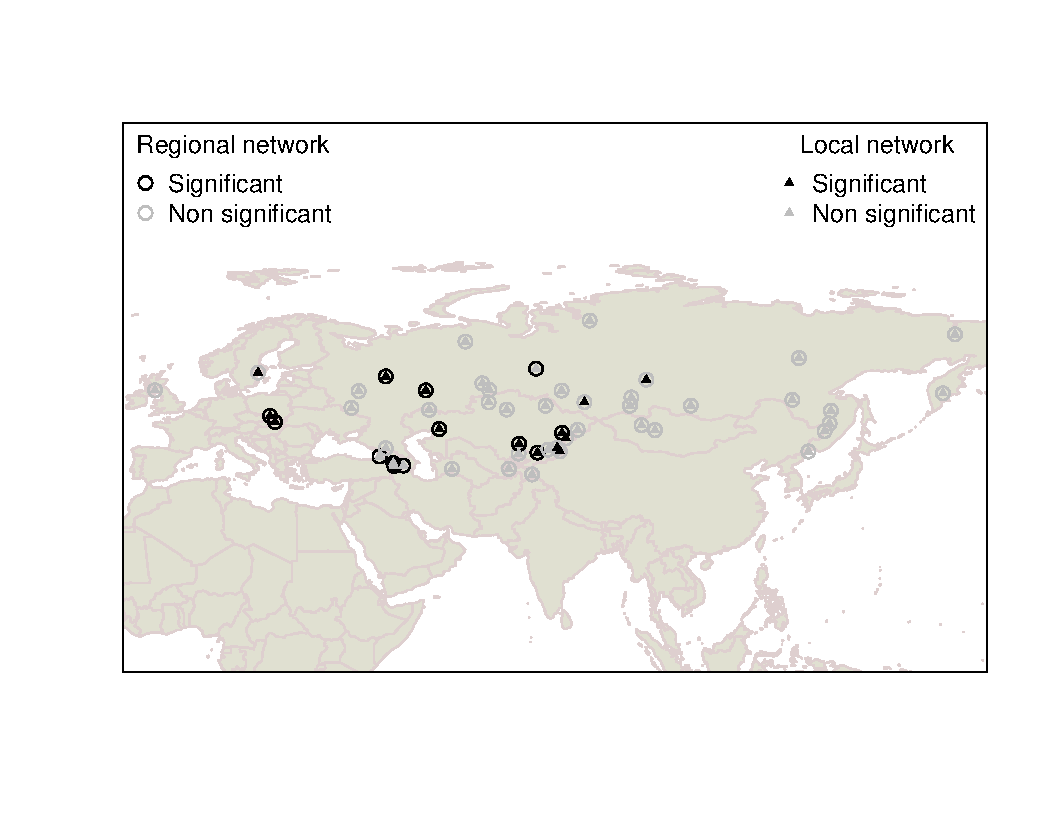
\includegraphics[width=\textwidth]{figure1.pdf}
\caption{Spatial distribution of coevolutionary signal across the 51
sites. For each location, we indicate whether or not the structure of
regional and local interaction networks is consistent with phylogenetic
congruence. The colour of the circle corresponds to regionally
significant or non-significant (black and grey, respectively) while the
colour of the symbol within corresponds to locally significant or
non-significant (black and grey, respectively).}
\end{figure}

\clearpage

\begin{figure}[p]
\centering
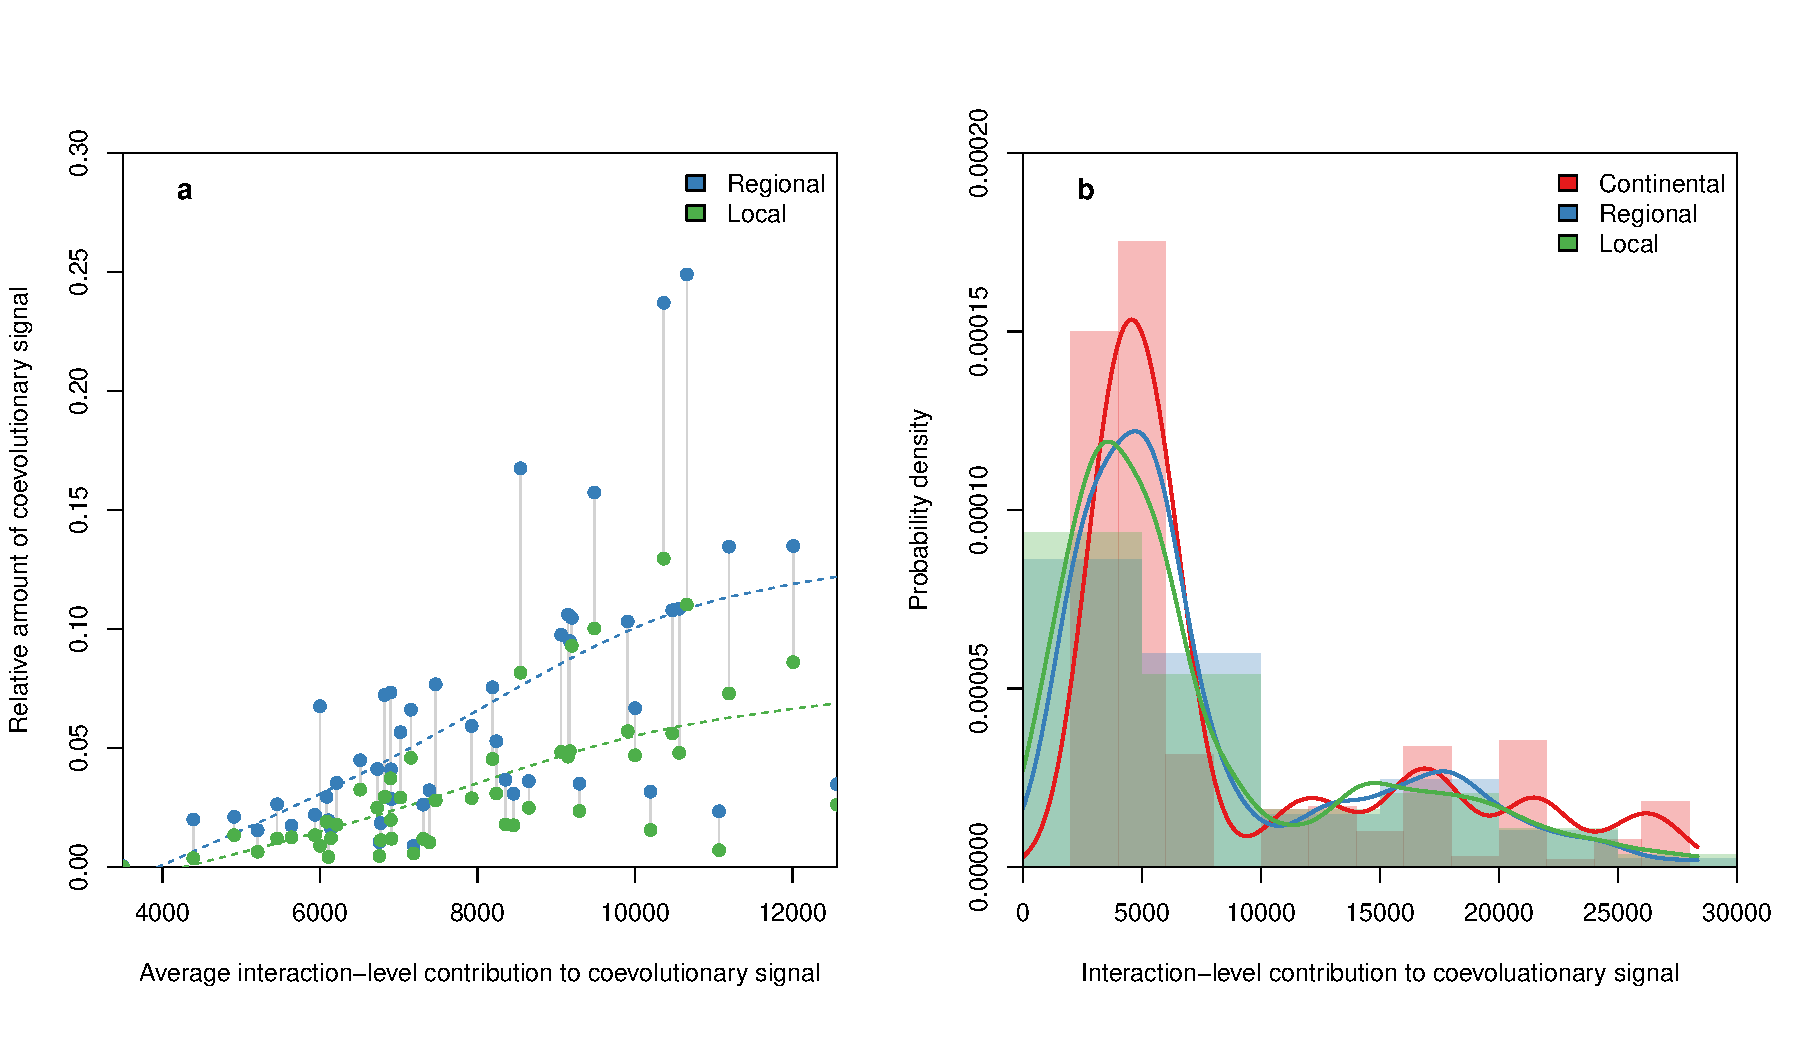
\includegraphics[width=\textwidth]{figure4.pdf}
\caption{Distribution of coevolutionary signal at the network and
interaction levels. \textbf{a}, Networks that have lower coevolutionary
signal at the local or regional level are composed of interactions that
on average contribute little to coevolution at the continental scale.
Dashed lines are the cubic smoothing spline; the two levels of the same
networks are linked by solid grey lines. \textbf{b}, Overall,
interactions observed at the local, regional, and continental scale have
equal contributions to coevolutionary signal. Probability density was
smoothed using a Gaussian kernel density estimator. Raw probability
densities are shown as semi-transparent bars.}
\end{figure}

\clearpage

\begin{figure}[p]
\centering
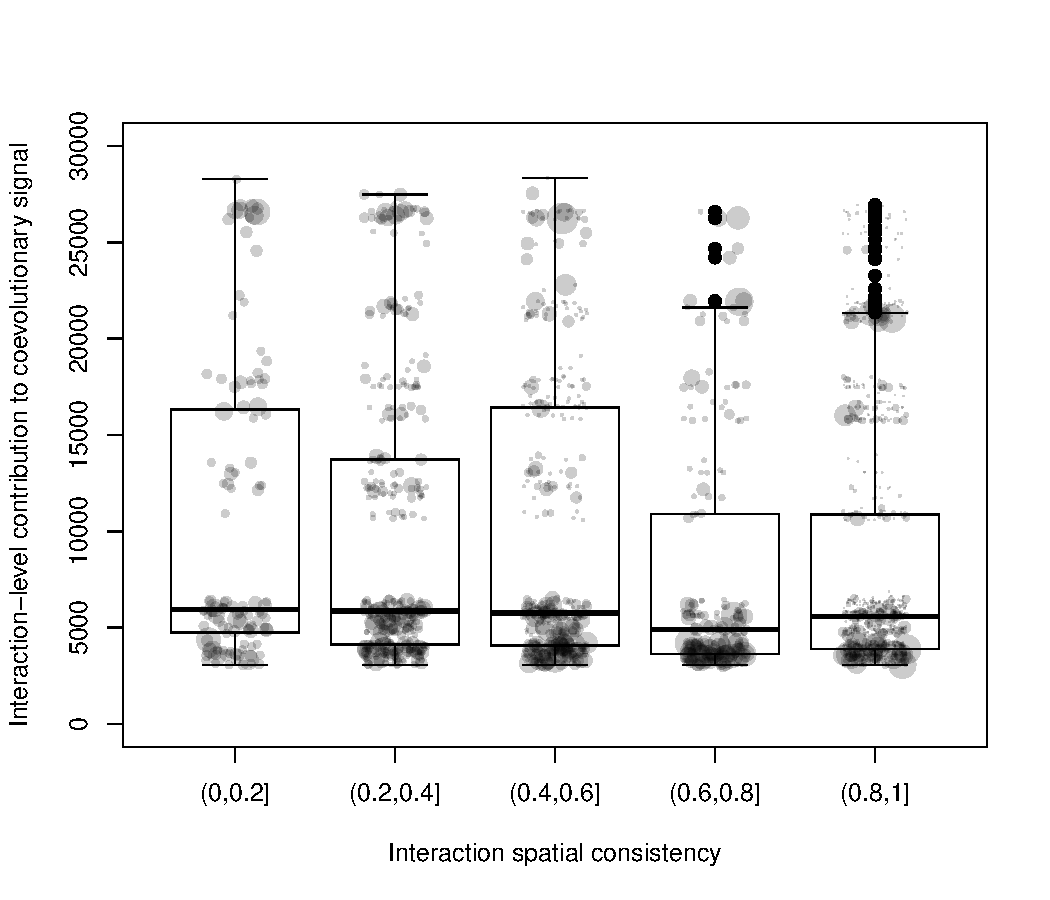
\includegraphics[width=\textwidth]{figure3.pdf}
\caption{Spatial consistency of an interaction and its contribution to
coevolutionary signal. Spatial consistency is defined as the probability
of observing an interaction between two species given that they were
observed to co-occur. Although statistically significant, there was no
biologically meaningful relationship between spatial consistency and an
interaction's importance for coevolution in the continental network
(\(R^2 \approx 0.01\), \(\rho = -0.1\), \(p \leq 10^{-5}\)).}
\end{figure}

\clearpage

\begin{figure}[p]
\centering
\includegraphics[width=\textwidth]{figure2.pdf}
\caption{The contribution to coevolutionary signal of the interaction
between two species is maintained across scales. For every site, we show
the Pearson's correlation between interaction-level coevolutionary
signal in the continental network and the same in the local network. The
size of each point is proportional to the size of the network, and all
correlations are significant at \(\alpha = 0.05\) except in the grey
shaded area.}
\end{figure}

\end{document}


